% \input{values/article-discussion.tex}

\section{Results}

% repeat hypothesis in operationalized terms
% describe analytic plan

\subsection{figure}

See Figure~\ref{fig:tavernier-blue}.

\begin{figure}[!ht]
    \centering
    {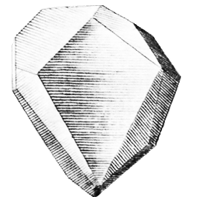
\includegraphics[width=3.5in]{graphics/tavernier-blue.png}}
    \caption{The Tavernier Blue.}
    \label{fig:tavernier-blue}
\end{figure}

\subsection{table}

See Table~\ref{fig:tabular-results}.

\begin{table}[htp]
\label{fig:tabular-results}
\caption{Tabular results}
\begin{tabular}{p{1.25in}p{1.25in}p{1.25in}}
\toprule
name & column 1 & column 2 \\
\midrule
first name & $p=0.0001$ & $20.0$ \\
second name & $p=ns$ & $40.0$ \\
third name & $p=ns$ & $60.0$
\end{tabular}
\end{table}
